\documentclass[11pt]{article}

% my added packages: copied from the swiss IJ paper
\usepackage{microtype}
\usepackage{graphicx}
\usepackage{subfigure}
\usepackage{booktabs} % for professional tables
\usepackage{siunitx}
\usepackage{hyperref}
\usepackage{xargs}[2008/03/08]

% Documentation
% http://ftp.math.purdue.edu/mirrors/ctan.org/macros/latex/contrib/refstyle/refstyle.pdf
\usepackage{refstyle}
\usepackage{varioref} % Use refstyle instead of varioref directly.
\usepackage[authoryear]{natbib}

\usepackage{amsmath}
\usepackage{amssymb}
\usepackage{amsfonts}
\usepackage{amsthm}
\usepackage{mathrsfs}
\usepackage{mathtools}
\usepackage{algpseudocode, algorithm} %typical alg typesetting packages

\usepackage{listings}
\usepackage{pdfpages}

% This picks up the knitr boilerplate, allowing us to \input partial knitr
% documents.
% This file contains the boilerplate that knitr would put at the top of
% a knitr document if you ran knitr with \begin{document} ... \end{document}.
% By including it once in the main document, you can knit and \input{}
% Rnw files that contain only individual sections.

\usepackage[]{graphicx}
\usepackage[]{color}
%% maxwidth is the original width if it is less than linewidth
%% otherwise use linewidth (to make sure the graphics do not exceed the margin)
\makeatletter
\def\maxwidth{ %
  \ifdim\Gin@nat@width>\linewidth
    \linewidth
  \else
    \Gin@nat@width
  \fi
}
\makeatother

\definecolor{fgcolor}{rgb}{0.345, 0.345, 0.345}
\newcommand{\hlnum}[1]{\textcolor[rgb]{0.686,0.059,0.569}{#1}}%
\newcommand{\hlstr}[1]{\textcolor[rgb]{0.192,0.494,0.8}{#1}}%
\newcommand{\hlcom}[1]{\textcolor[rgb]{0.678,0.584,0.686}{\textit{#1}}}%
\newcommand{\hlopt}[1]{\textcolor[rgb]{0,0,0}{#1}}%
\newcommand{\hlstd}[1]{\textcolor[rgb]{0.345,0.345,0.345}{#1}}%
\newcommand{\hlkwa}[1]{\textcolor[rgb]{0.161,0.373,0.58}{\textbf{#1}}}%
\newcommand{\hlkwb}[1]{\textcolor[rgb]{0.69,0.353,0.396}{#1}}%
\newcommand{\hlkwc}[1]{\textcolor[rgb]{0.333,0.667,0.333}{#1}}%
\newcommand{\hlkwd}[1]{\textcolor[rgb]{0.737,0.353,0.396}{\textbf{#1}}}%
\let\hlipl\hlkwb

\usepackage{framed}
\makeatletter
\newenvironment{kframe}{%
 \def\at@end@of@kframe{}%
 \ifinner\ifhmode%
  \def\at@end@of@kframe{\end{minipage}}%
  \begin{minipage}{\columnwidth}%
 \fi\fi%
 \def\FrameCommand##1{\hskip\@totalleftmargin \hskip-\fboxsep
 \colorbox{shadecolor}{##1}\hskip-\fboxsep
     % There is no \\@totalrightmargin, so:
     \hskip-\linewidth \hskip-\@totalleftmargin \hskip\columnwidth}%
 \MakeFramed {\advance\hsize-\width
   \@totalleftmargin\z@ \linewidth\hsize
   \@setminipage}}%
 {\par\unskip\endMakeFramed%
 \at@end@of@kframe}
\makeatother

\definecolor{shadecolor}{rgb}{.97, .97, .97}
\definecolor{messagecolor}{rgb}{0, 0, 0}
\definecolor{warningcolor}{rgb}{1, 0, 1}
\definecolor{errorcolor}{rgb}{1, 0, 0}
\newenvironment{knitrout}{}{} % an empty environment to be redefined in TeX

\usepackage{alltt}


% This defines math macros.
% Math definitions

% Some definitions for the text

\def\loset{MIS}
\def\loeff{MIP}
\def\loalpha{PIP}
\def\aloset{AMIS}
\def\aloeff{AMIP}
\def\aloalpha{APIP}
\def\na{\texttt{NA}}

%%%%%%%%%%%%%%%%%%%%%%%%
% Rachael's math defs

\DeclareMathOperator*{\argmax}{arg\,max}
\DeclareMathOperator*{\argmin}{arg\,min}

\DeclarePairedDelimiter\abs{\lvert}{\rvert}
\DeclarePairedDelimiter\norm{\lVert}{\rVert}

% Swap the definition of \abs* and \norm*, so that \abs
% and \norm resizes the size of the brackets, and the
% starred version does not.
\makeatletter
\let\oldabs\abs
\def\abs{\@ifstar{\oldabs}{\oldabs*}}

%\let\oldnorm\norm
\def\norm{\@ifstar{\oldnorm}{\oldnorm*}}

%%%%%%%%%%%%%%%%%%%%%%%%
% Ryan's math defs


% \norm was taken, so use \vnorm for "vector norm".
\global\long\def\info{\mathcal{I}}%

% These are all used for the finite sample bounds section.
\global\long\def\betalin{\hat\beta^{\mathrm{lin}}}%
\global\long\def\nset{\mathcal{S}}%

\global\long\def\cop{C_{op}}%
\global\long\def\cmoment{H_2}%
\global\long\def\cxxlo{\xi_1}%
\global\long\def\cxepslo{\xi_2}%
\global\long\def\cball{\mathscr{B}}%
\global\long\def\cijdiff{\Delta_{lin}}%

\global\long\def\copscaled{\tilde{C}_{op}}%

% calculus
\newcommand{\dee}{\mathrm{d}}

% Influence score and related quantities
\def\infl{\psi}
\def\inflscale{\hat{\sigma}_{\infl}}
\def\inflscalelim{\sigma_{\infl}}
\def\ind#1{\mathbb{I}\left(#1\right)}
\def\mis#1{S_{#1}}
\def\mip#1{\Psi_{#1}}
\def\amis#1{\hat{S}_{#1}}
\def\amip#1{\hat{\Psi}_{#1}}
\def\loprop#1{\alpha^*_{#1}}
\def\aloprop#1{\hat{\alpha}^*_{#1}}
\def\thetafun{\phi}
\def\thetafunlin{\thetafun^{\mathrm{lin}}}%
\def\thetalin{\thetahat^{\mathrm{lin}}}%

\def\shape{\mathcal{S}_\alpha}
\def\noise{\hat\sigma_{\phi}}
\def\plim{\overset{p}{\rightarrow}}

% Vectors
%\def\x{\vec{x}}
\def\d{d} % A general data point
\def\p{p} % The index into the parameter vector
\def\P{P} % The length of the parameter vector
\def\w{\vec{w}}
\def\wnorm{\vec{\omega}} % Used only in the \thetafun lemma

\def\zP{0_{\P}}
\def\zPN{0_{\P \times N}}
\def\thetahat{\hat{\theta}}
\def\onevec{\vec{1}}
\def\inflvec{\vec{\infl}}

% Operators
\def\sumn{\sum_{n=1}^N}
\def\meann{\frac{1}{N}\sum_{n=1}^N}
\def\var#1{\mathrm{Var}\left(#1\right)}
\def\vnorm#1{\left\Vert #1\right\Vert }%
\def\falphanorm#1#2{\left\Vert #2\right\Vert_{#1, \alpha} }%
\def\at#1#2{\left.#1\right|_{#2}}%
\def\fracat#1#2#3{\at{\frac{#1}{#2}}{#3}}%
\def\mbe{\mathbb{E}}%
\def\argmaxover#1{\underset{#1}{\mathrm{argmax}}\,}
\def\maxover#1{\underset{#1}{\mathrm{max}}\,}


% This specifies the formatting for references (sections, theorems, etc.)

%%%%%%%%%%%%%%%%%%%%
% amsthm commands

\theoremstyle{plain}
\newtheorem{lem}{Lemma}
\newtheorem{thm}{Theorem}
\newtheorem{prop}{Proposition}
\newtheorem{cond}{Condition}
\newtheorem{assu}{Assumption}
\newtheorem{cor}{Corollary}
\newtheorem{conj}{Conjecture}

\theoremstyle{definition}
\newtheorem{defn}{Definition}
%\newtheorem{ex}{Example}

% Example environment with a terminating symbol.
% https://tex.stackexchange.com/questions/16453/denoting-the-end-of-example-remark
\theoremstyle{definition}
\newtheorem{examplex}{Example}
\newenvironment{ex}
  {\pushQED{\qed}\renewcommand{\qedsymbol}{$\triangle$}\examplex}
  {\popQED\endexamplex}


%%%%%%%%%%%%%%%%%%%%
% refstyle commands

\newref{event}{
    name=Event~, %
    names=Events~, %
    Name=Event~,
    Names=Events~
    }

\newref{item}{
    name=Item~, %
    names=Items~, %
    Name=Item~,
    Names=Items~
    }

\newref{fig}{
    name=Figure~, %
    Name=Figure~
    }

\newref{tab}{
    name=Table~, %
    Name=Table~
    }

\newref{sec}{
    name=Section~, %
    Name=Section~,
    names=Sections~, %
    Names=Sections~
    }

\newref{app}{
    name=Appendix~, %
    Name=Appendix~
    }

\newref{eq}{
    name=Eq.~, %
    Name=Eq.~,
    names=Eqs.~, %
    Names=Eqs.~
    }

\newref{fig}{
    name=Figure~, %
    Name=Figure~
    }

\newref{def}{
    name=Definition~, %
    Name=Definition~
    }

\newref{assu}{
    name=Assumption~, %
    Name=Assumption~,
    names=Assumptions~, %
    Names=Assumptions~,
    }

\newref{cond}{
    name=Condition~, %
    Name=Condition~,
    names=Conditions~, %
    Names=Conditions~
    }

\newref{prop}{
    name=Proposition~, %
    Name=Proposition~,
    names=Propositions~, %
    Names=Propositions~
    }

\newref{lem}{
    name=Lemma~, %
    Name=Lemma~,
    names=Lemmas~, %
    Names=Lemmas~
    }

\newref{ex}{
    name=Example~, %
    Name=Example~}

\newref{cor}{
    name=Corollary~, %
    Name=Corollary~
    }

\newref{thm}{
    name=Theorem~, %
    Name=Theorem~,
    names=Theorems~, %
    Names=Theorems~
    }

\newref{proof}{
    name=Proof~, %
    Name=Proof~
    }

\newref{conj}{
    name=Conjecture~, %
    Name=Conjecture~
    }

\newref{algr}{
    name=Algorithm~, %
    Name=Algorithm~,
    names=Algorithms~, %
    Names=Algorithms~,
    }


%% refstyle examples:
% \Secref[vref]{introduction} contains \secref{introduction}.
% \Secref[vref]{ack} does not contain \secref{introduction}.
%
% \begin{align}
%     x=y \eqlabel{myeq}
% \end{align}
%


\begin{document}

\title{Maybe You Should Use Knitr}

\author{Ryan Giordano \texttt{rgiordan@mit.edu}}

\maketitle

\begin{abstract}
This is an abstract.
\end{abstract}

\section{Introduction}\seclabel{introduction}

\begin{frame}{Mister freakin P}


\end{frame}





\section{Experiment One}\seclabel{experiement_one}
% experiment_one.tex is generated by knitr
%%%%%%%%%%%%%%%%%%%%%%%%%%%%%%%%%%%%%%
%%%%%%%%%%%%%%%%%%%%%%%%%%%%%%%%%%%%%%
% Do not edit the TeX file your work
% will be overwritten.  Edit the RnW
% file instead.
%%%%%%%%%%%%%%%%%%%%%%%%%%%%%%%%%%%%%%
%%%%%%%%%%%%%%%%%%%%%%%%%%%%%%%%%%%%%%





\newcommand{\EoneNumObs}{1,000}


We generated $\EoneNumObs$ observations.  They looked like a mess,
as you can see in \figref{eone_scatter}.


\begin{knitrout}
\definecolor{shadecolor}{rgb}{0.969, 0.969, 0.969}\color{fgcolor}\begin{figure}[!h]

{\centering 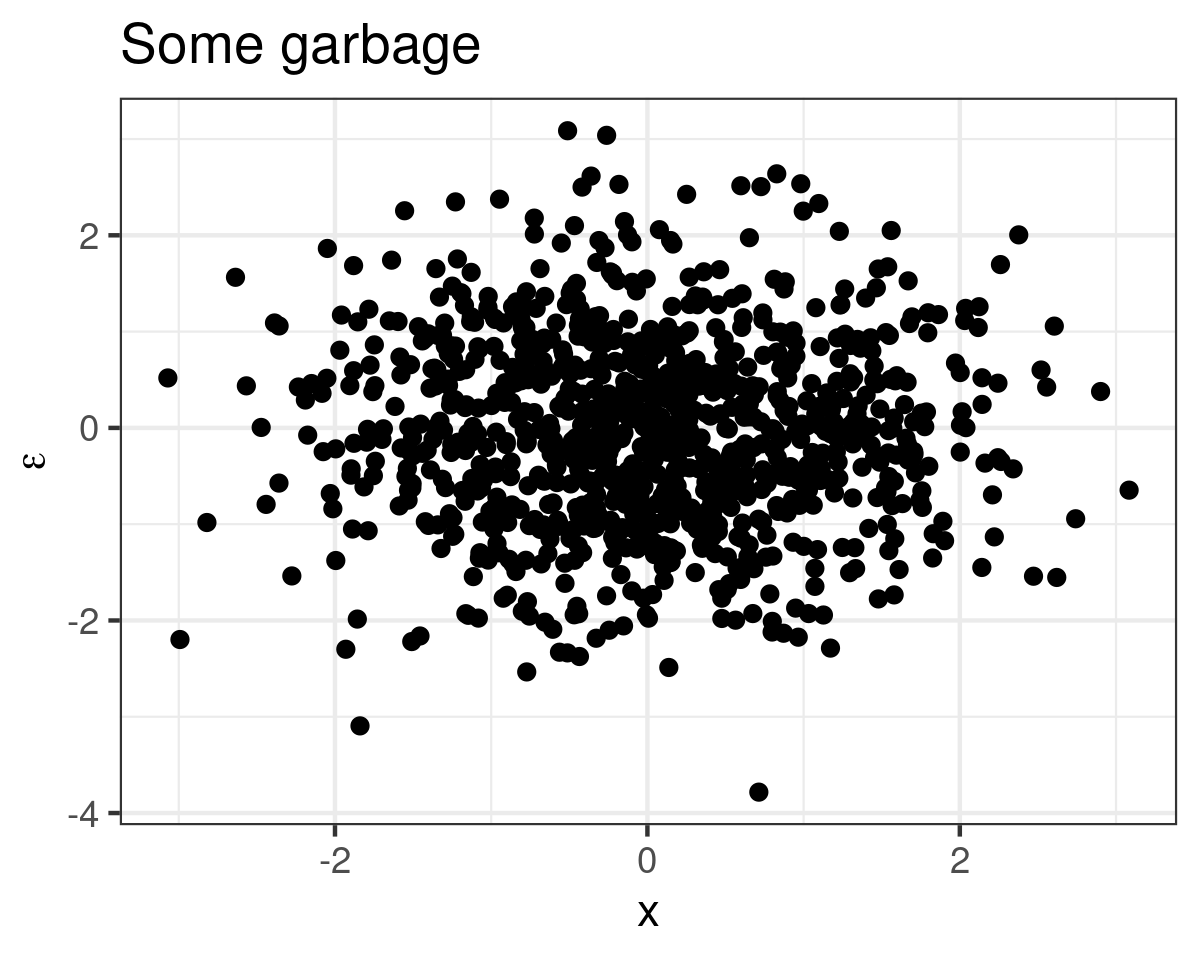
\includegraphics[width=0.980\linewidth,height=0.784\linewidth]{figure/eone_scatter-1} 

}

\caption[It's nice to have a long figure caption that allows easy access to latex stuff like there were $\EoneNumObs$ draws of $x$ and $\epsilon$ that went into this plot]{It's nice to have a long figure caption that allows easy access to latex stuff like there were $\EoneNumObs$ draws of $x$ and $\epsilon$ that went into this plot.}\label{fig:eone_scatter}
\end{figure}


\end{knitrout}

And \figref{eone_hist} as well.  What garbage.


\begin{knitrout}
\definecolor{shadecolor}{rgb}{0.969, 0.969, 0.969}\color{fgcolor}\begin{figure}[!h]

{\centering 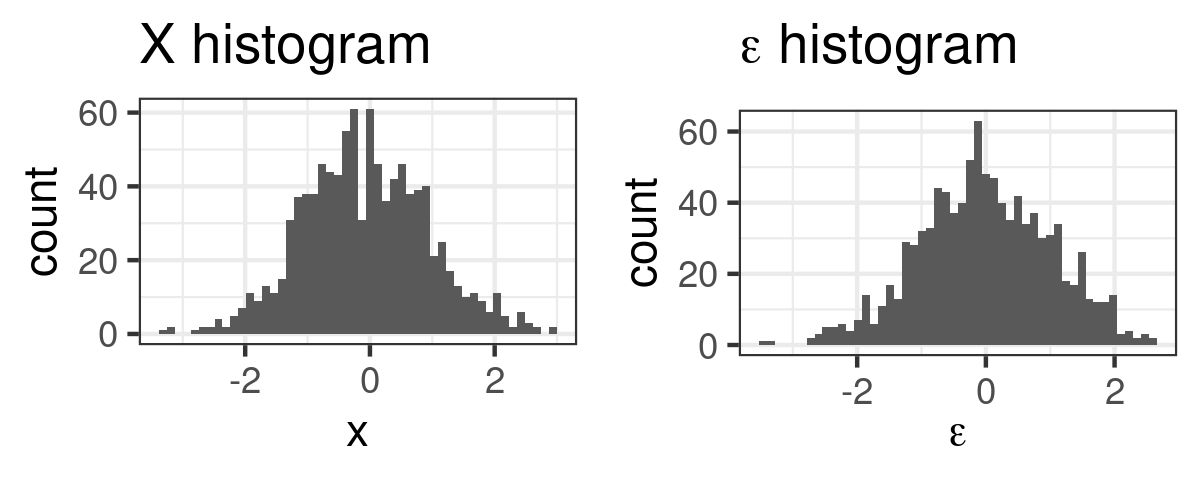
\includegraphics[width=0.980\linewidth,height=0.392\linewidth]{figure/eone_hist-1} 

}

\caption[You can reuse this variable for other captions]{You can reuse this variable for other captions.}\label{fig:eone_hist}
\end{figure}


\end{knitrout}
%


\section{Experiment Two}\seclabel{experiement_two}
% experiment_two.tex is generated by knitr
%%%%%%%%%%%%%%%%%%%%%%%%%%%%%%%%%%%%%%
%%%%%%%%%%%%%%%%%%%%%%%%%%%%%%%%%%%%%%
% Do not edit the TeX file your work
% will be overwritten.  Edit the Rnw
% file instead.
%%%%%%%%%%%%%%%%%%%%%%%%%%%%%%%%%%%%%%
%%%%%%%%%%%%%%%%%%%%%%%%%%%%%%%%%%%%%%





\newcommand{\ETwoNumObs}{1,000}
\newcommand{\ETwoBeta}{5}


We generated $\ETwoNumObs$ observations again, but now we used an offset $\beta =
\ETwoBeta$.  They looked better, but we already showed you how to make a graph,
so instead we'll show it in \tabref{amazing_table}.


\begin{table}[h]
\begin{center}% latex table generated in R 3.6.3 by xtable 1.8-4 package
% Fri Apr  9 19:40:17 2021
\begin{tabular}{lrr}
  \hline
metric & x & y \\ 
  \hline
mean & -0.0751 & -0.3913 \\ 
  sd & 1.0112 & 5.2012 \\ 
  max & 2.9757 & 16.0883 \\ 
   \hline
\end{tabular}
\end{center}
\caption{Amazing summary stats\tablabel{amazing_table}}
\end{table}


\bibliography{references}
\end{document}
